\documentclass{beamer}
\usepackage[latin1]{inputenc}
\usepackage[francais]{babel}
\usepackage{graphicx}
\usepackage{default}
\usepackage{amsfonts,amssymb}


\title{Structuring the Synthesis of Heap-Manipulating Programs}

\author{NADIA POLIKARPOVA, UCSD, USA \\ILYA SERGEY, University College London, UK}

\date{}
\begin{document}
	\maketitle
\begin{frame}[fragile]
	\frametitle{Introduction}
	
	\begin{center}
		
\includegraphics[height=\baselineskip]{figures/swap.png}
	\end{center}
	\textbf{Int�r�t} : Faire avancer l'�tat de l'art en mati�re de synth�se de programmes qui manipulent des pointeurs � partir de sp�cifications fonctionelles formelles.\\
	\textbf{Id�e Cl�} : Utiliser la logique de s�paration.\\
	\textbf{Contributions} : Synthetic Separation Logic un systeme de preuve. Et SuSLik leur synth�tiseur
\end{frame}
\begin{frame}[fragile]
	\frametitle{Sp\'ecifications pour la Synth\`ese}
	On utilise ici des tas symboliques.\\
	\begin{center}
	$\mathrm{\Sigma};\mathrm{\Gamma};\{\mathcal{P}\}\leadsto\{\mathcal{Q}\} | c$
	\end{center}
	\begin{itemize}
		\item $\mathrm{\Gamma}$ : environnement
		\item $\mathrm{\Sigma}$ : contexte
		\item $\mathcal{P}$,$\phi$,P : pr�condition, ses parties pure et spatiale
		\item $\mathcal{Q}$,$\psi$,Q : postcondition, ses parties pure et spatiale
		\item $GV(\mathrm{\Gamma},\mathcal{P},\mathcal{Q}) = Vars(\mathcal{P}) \backslash \mathrm{\Gamma}$ 
		\item $EV(\mathrm{\Gamma},\mathcal{P},\mathcal{Q}) = Vars(\mathcal{Q}) \backslash (\mathrm{\Gamma} \cup Vars(\mathcal{P})$ 
	\end{itemize}
\end{frame}
\begin{frame}[fragile]
	\frametitle{R�gles d'Inf�rence Basiques}
	\framesubtitle{Un exemple}
	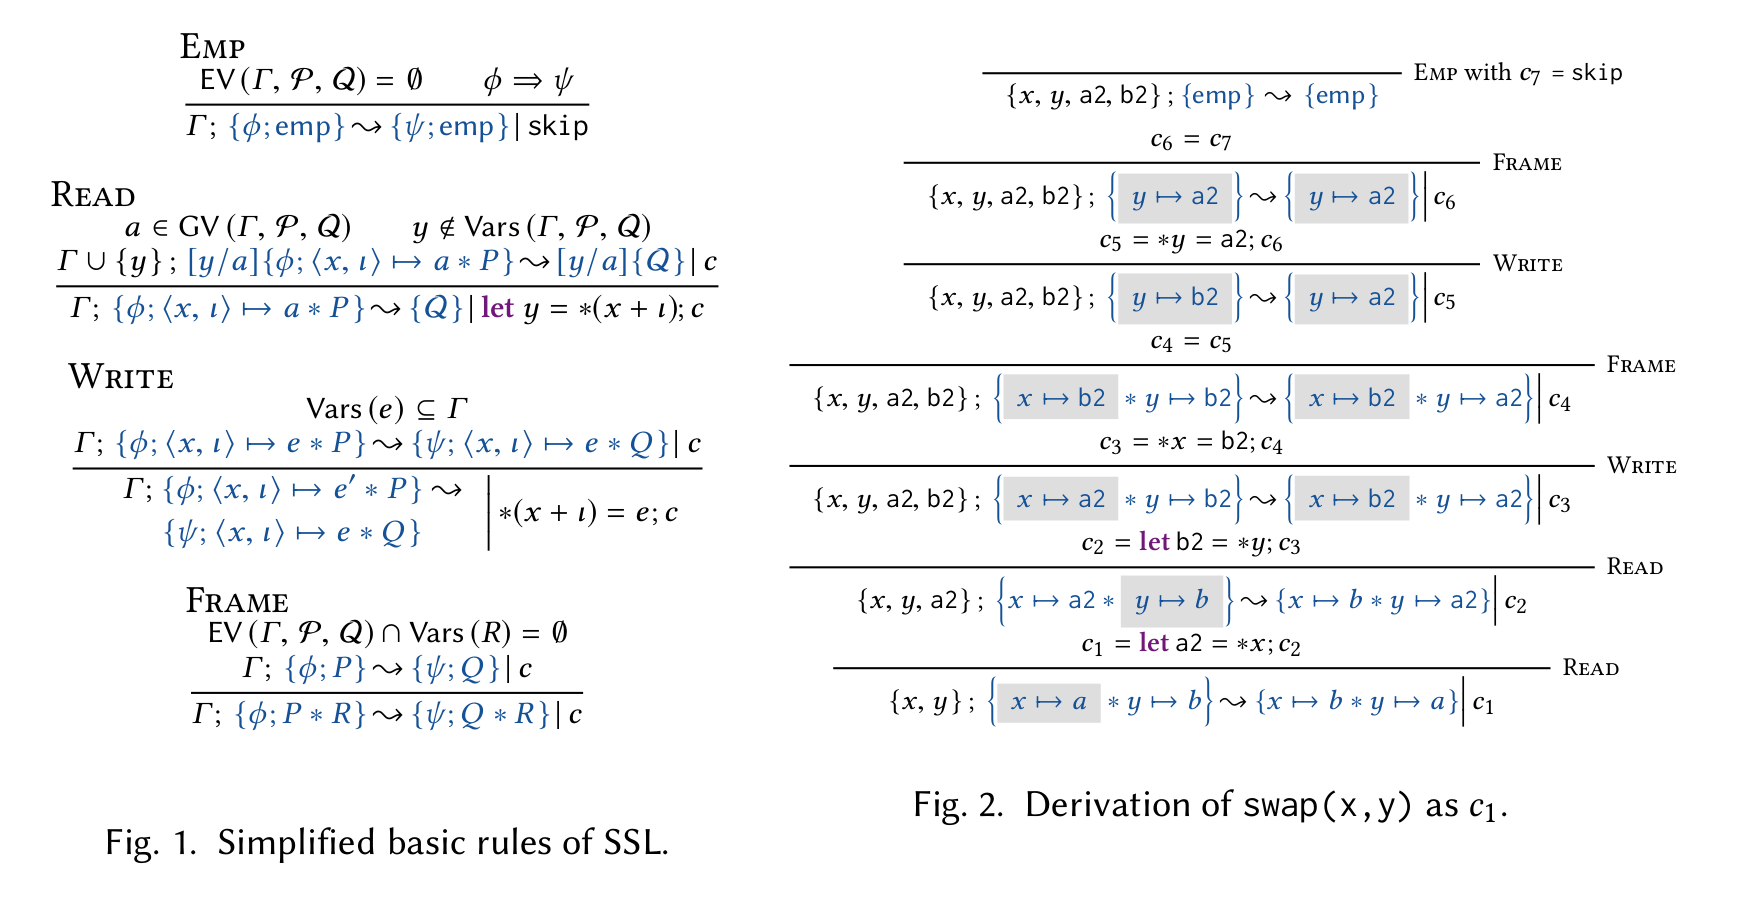
\includegraphics[width=11cm]{figures/basic.png}
\end{frame}
\begin{frame}
	\frametitle{R�gles d'Inf�rence Basiques}
	\begin{itemize}
		\item[EMP] terminale, parties spatiales vide, $EV = \emptyset$, $\phi \implies \psi$ \\ skip
		\item[READ] assigne la valeur d'une GV a une nouvelle variable de programme et substitue toutes les occurences.\\
		let b = *x
		\item[WRITE] assigne l'�valuation d'une expression e � une case m�moire.\\
		*x = b 
		\item[FRAME] Enl�ve une partie spatiale commune � $\phi$ et $\psi$, si cela ne cr�e pas de variable existentielle.\\
		skip
	\end{itemize}
\end{frame}
\begin{frame}[fragile]
	\frametitle{Unification Spatiale et Backtrack}
\end{frame}
\begin{frame}[fragile]
	\frametitle{Raisonner sur les contraintes pures}
	\framesubtitle{Pr\'econditions}
\end{frame}
\begin{frame}[fragile]
	\frametitle{Raisonner sur les contraintes pures}
	\framesubtitle{Postconditions}
\end{frame}
\begin{frame}[fragile]
	\frametitle{Synth\`ese pour pr\'edicats inductifs}
	\framesubtitle{M\'emoire dynamique}
\end{frame}
\begin{frame}[fragile]
	\frametitle{Synth\`ese pour pr\'edicats inductifs}
	\framesubtitle{Induction}
\end{frame}
\begin{frame}[fragile]
	\frametitle{Synth\`ese pour pr\'edicats inductifs}
	\framesubtitle{D\'eroulement de pr\'edicat}
\end{frame}
\begin{frame}[fragile]
	\frametitle{Synth\`ese pour pr\'edicats inductifs}
	\framesubtitle{Etiquette de niveau}
\end{frame}
\begin{frame}[fragile]
	\frametitle{Synth\`ese pour pr\'edicats inductifs}
	\framesubtitle{D\'eroulement dans la postcondition}
\end{frame}
\begin{frame}[fragile]
	\frametitle{Permettre l'appel de proc\`edure}
	\framesubtitle{Enl\'evement de l'appel}
\end{frame}
\begin{frame}[fragile]
	\frametitle{Synthetic Separation Logic}
	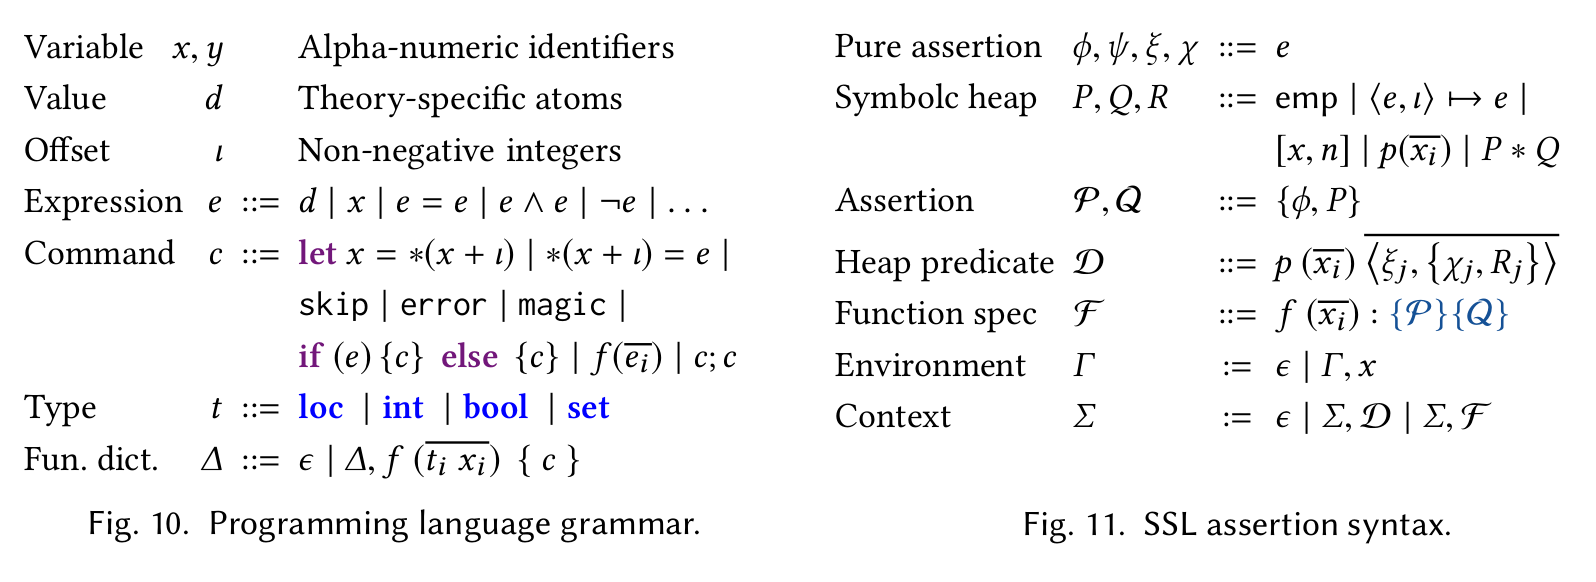
\includegraphics[width=11cm]{figures/syntax.png}
\end{frame}
\begin{frame}[fragile]
	\frametitle{Synthetic Separation Logic}
	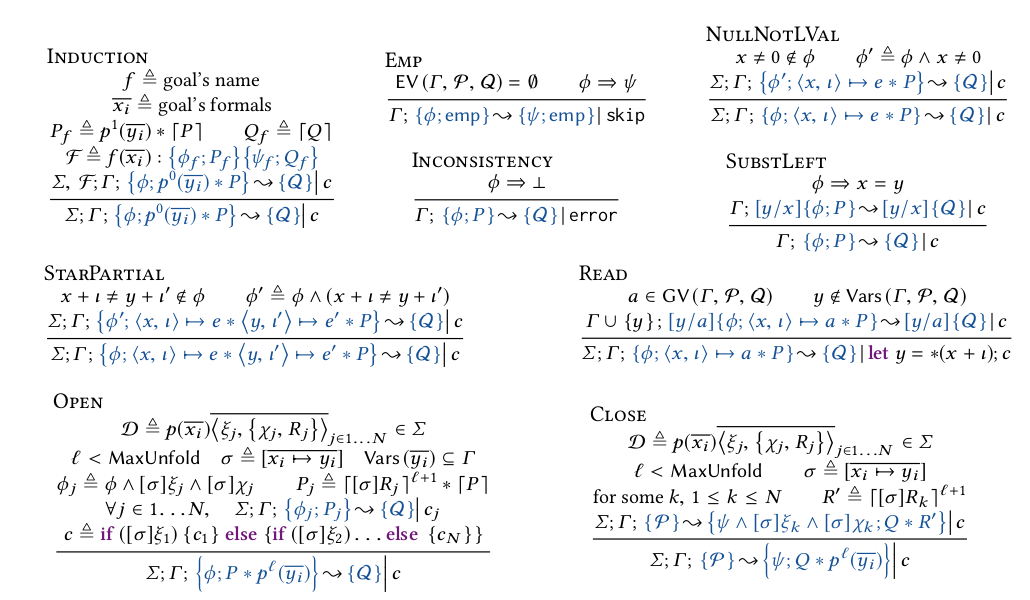
\includegraphics[width=11cm]{figures/zoo1.png}
\end{frame}
\begin{frame}[fragile]
	\frametitle{Synthetic Separation Logic}
	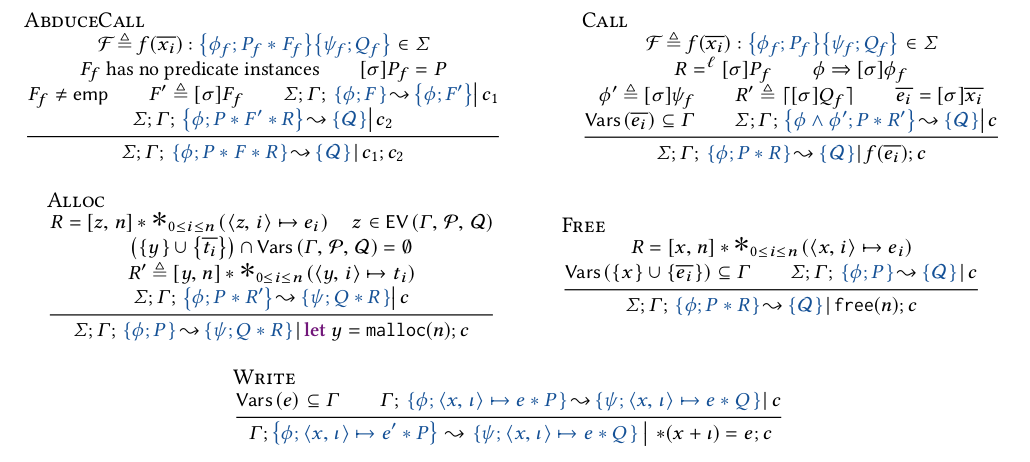
\includegraphics[width=11cm]{figures/zoo2.png}
\end{frame}
\begin{frame}[fragile]
	\frametitle{Synthetic Separation Logic}
	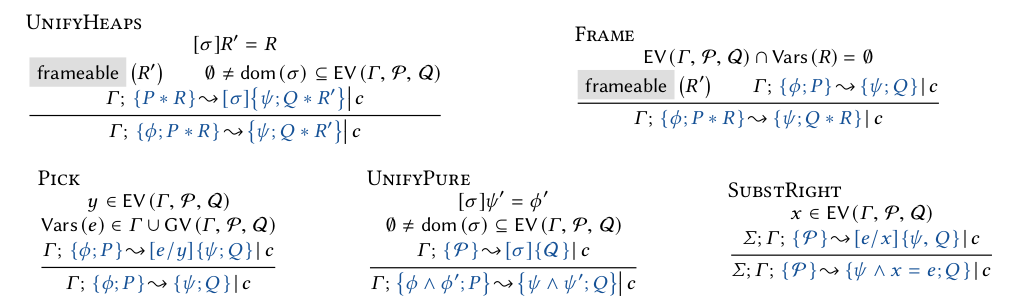
\includegraphics[width=11cm]{figures/zoo3.png}
\end{frame}
\begin{frame}[fragile]
	\frametitle{Garanties Formelles}
	La validit� pour la partie SL est assez similaire au cas plus classique.\\
	\vspace{0.5cm}
	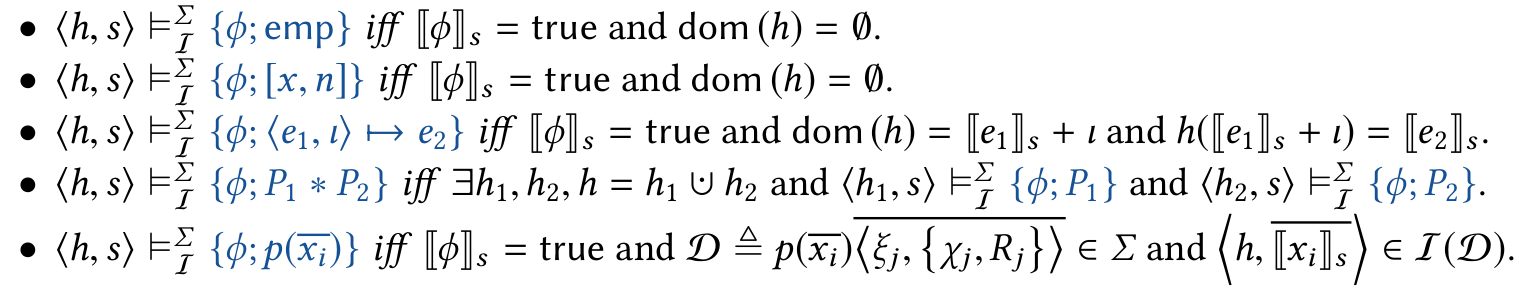
\includegraphics[width=11cm]{figures/satisfaction.png}
\end{frame}
\begin{frame}[fragile]
	\frametitle{Garanties Formelles}
	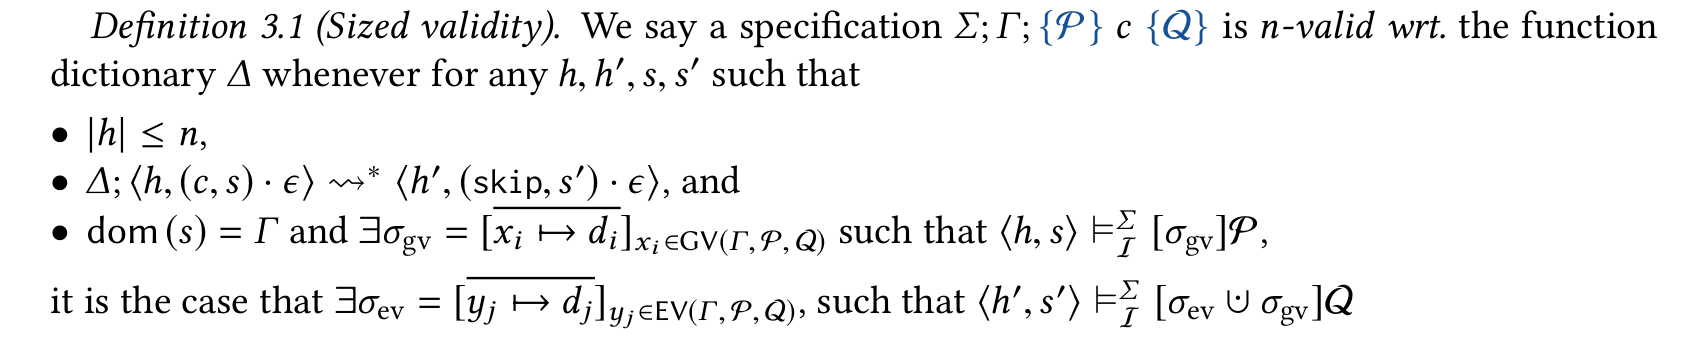
\includegraphics[width=11cm]{figures/nvalid.png}\\
	
	On d�finit une correction vis � vis de la pr� et post condition mais seulement pour des tas de taille n.
\end{frame}
\begin{frame}[fragile]
	\frametitle{Garanties Formelles}
	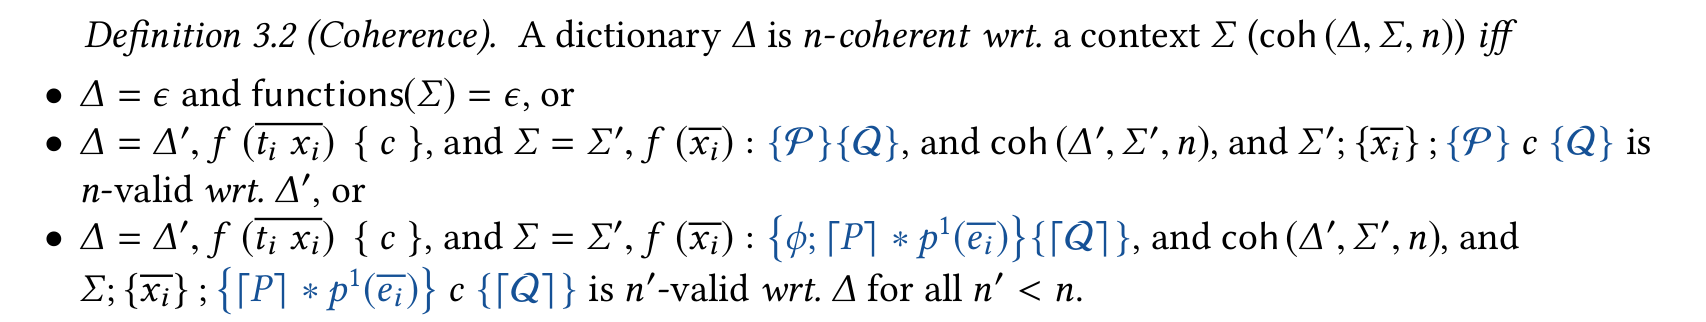
\includegraphics[width=11cm]{figures/coherence.png}
\end{frame}
\begin{frame}[fragile]
	\frametitle{Garanties Formelles}
	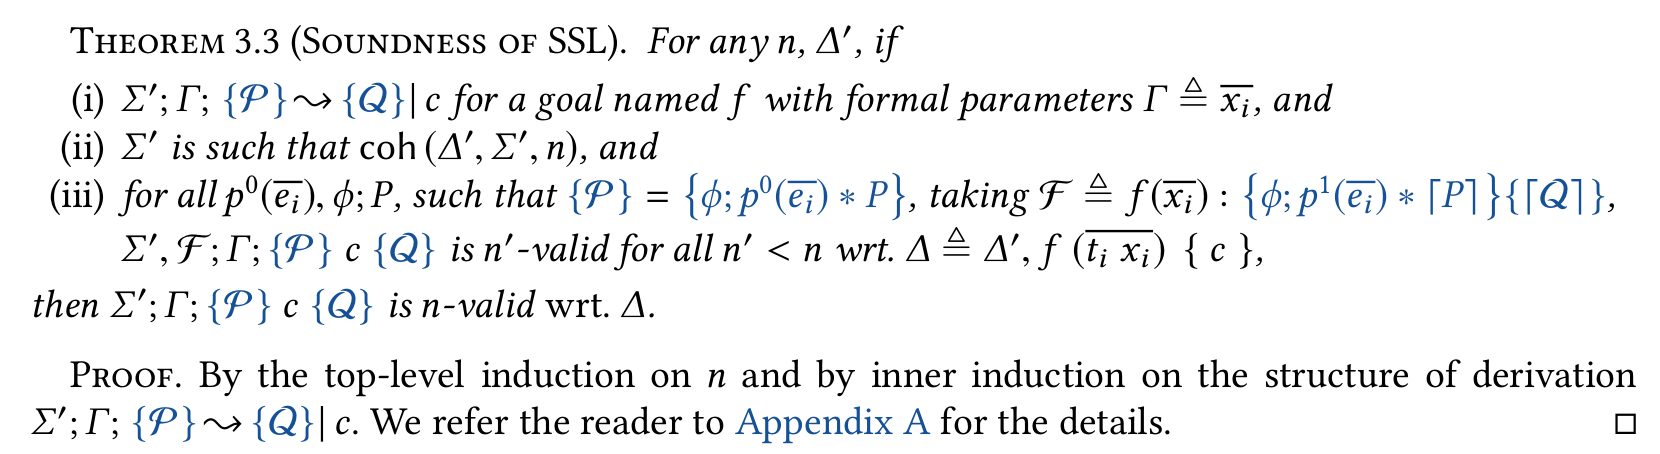
\includegraphics[width=11cm]{figures/thm.png}
\end{frame}
\begin{frame}[fragile]
	\frametitle{Algorithme de synth\`ese bas\'e sur SSL}
\end{frame}
\begin{frame}[fragile]
	\frametitle{Optimisations et extensions}
	Optimisations :
	\begin{itemize}
		\item R\`egles inversibles
		\pause
		\item Recherche multi-phase
		\pause
		\item R\`eduction des sym\'etries
		\pause
		\item R\`egles d'\'echec 
	\end{itemize}
	\pause
	Extensions :
	\begin{itemize}
	\item Fonctions auxilliaire
	\pause
	\item Enl\`evement de branches	
	\end{itemize}
\end{frame}
\begin{frame}
	\frametitle{Benchmark}
	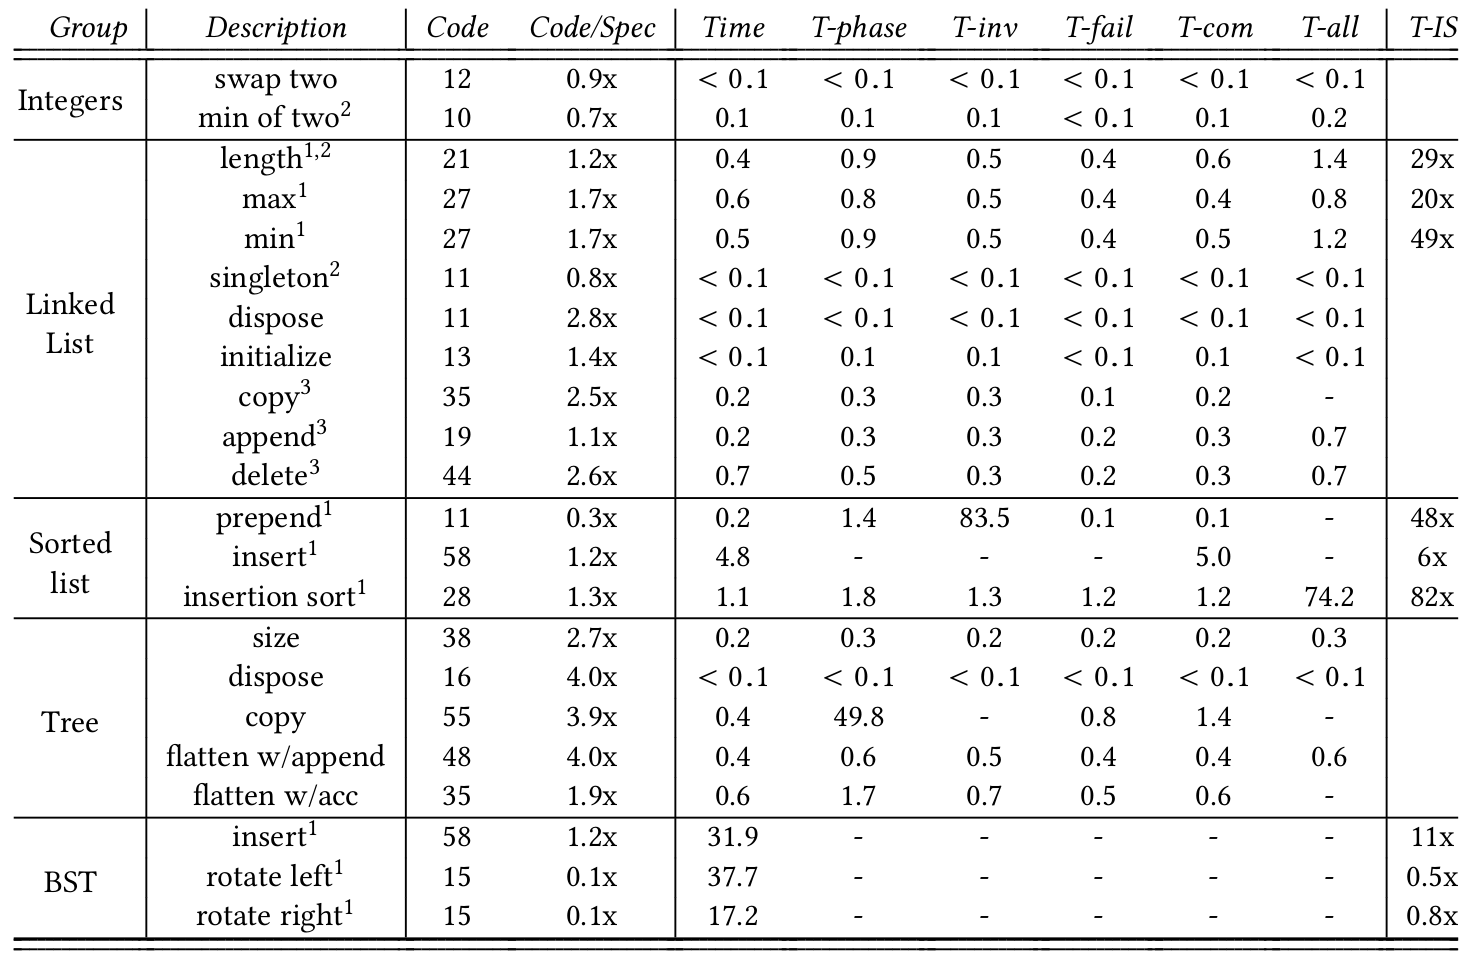
\includegraphics[width=11cm]{figures/benchmark.png}
\end{frame}


\end{document}
